\documentclass[xcolor=dvipsnames,10pt,aspectratio=169]{beamer}
%\documentclass[xcolor=dvipsnames,10pt]{beamer}
\usepackage{etex}
\usepackage{pgf,pgfarrows,pgfnodes,pgfautomata,pgfheaps,pgfshade}
\usepackage[absolute,overlay]{textpos} 
%\usepackage{algorithm}
\usepackage{amsmath,amssymb}
\usepackage[utf8]{inputenc} 
\usepackage{colortbl}
\usepackage{graphicx} 
\usepackage[brazil]{babel}
\usepackage{tabularx} 
\usepackage{multirow}
\usepackage{booktabs}
\usepackage{listings}
%\usepackage{multimedia}
\usepackage{animate}
\usepackage{xcolor}
\usepackage{array}
\usepackage{longtable}
\usepackage{makecell}
\usepackage{caption}
\usetheme{Madrid} 
\usepackage{amsmath}
\usepackage{movie15}


\lstset{ %
%	backgroundcolor=\color{white},   % choose the background color; you must add \usepackage{color} or \usepackage{xcolor}
%	basicstyle=\footnotesize,        % the size of the fonts that are used for the code
	basicstyle=\scriptsize,        % the size of the fonts that are used for the code
	breakatwhitespace=false,         % sets if automatic breaks should only happen at whitespace
	breaklines=true,                 % sets automatic line breaking
	captionpos=t,                    % sets the caption-position to bottom
	commentstyle=\color{mygreen},    % comment style
	deletekeywords={...},            % if you want to delete keywords from the given language
	escapeinside={\%*}{*)},          % if you want to add LaTeX within your code
	extendedchars=true,              % lets you use non-ASCII characters; for 8-bits encodings only, does not work with UTF-8
%	frame=single,                    % adds a frame around the code
	keepspaces=true,                 % keeps spaces in text, useful for keeping indentation of code (possibly needs columns=flexible)
	keywordstyle=\color{blue},       % keyword style
%	language=make,                 % the language of the code
	morekeywords={*,...},            % if you want to add more keywords to the set
%	numbers=left,                    % where to put the line-numbers; possible values are (none, left, right)
%	numbersep=5pt,                   % how far the line-numbers are from the code
	numberstyle=\tiny\color{mygray}, % the style that is used for the line-numbers
	rulecolor=\color{black},         % if not set, the frame-color may be changed on line-breaks within not-black text (e.g. comments (green here))
	showspaces=false,                % show spaces everywhere adding particular underscores; it overrides 'showstringspaces'
	showstringspaces=false,          % underline spaces within strings only
	showtabs=false,                  % show tabs within strings adding particular underscores
	stepnumber=2,                    % the step between two line-numbers. If it's 1, each line will be numbered
}

\definecolor{mygreen}{rgb}{0,0.6,0}
\definecolor{mygray}{rgb}{0.5,0.5,0.5}
\definecolor{mymauve}{rgb}{0.58,0,0.82}

\usecolortheme{beaver}
\newcommand{\ul}{\underline}
\setbeamertemplate{footline}{\scriptsize{\vspace*{0.3cm}\hspace*{15cm}\insertframenumber\,/\,\inserttotalframenumber}}
\setbeamertemplate{caption}[numbered]
\setbeamerfont{caption}{size=\fontsize{8}{5}}

\setbeamercolor{block title}{	bg=Sepia , fg = White}
\setbeamercolor{block body}{bg=Brown!15, fg=Sepia }
\setbeamercolor{item projected}{bg=Sepia, fg=White}
\setbeamercolor{number projected}{bg = Black}

%declara as imagens usadas no layout do slide
\pgfdeclareimage[height=0.8cm]{mflab}{figuras/logo_mflab_transparente.png}
\pgfdeclareimage[height=1.0cm]{logoufu}{figuras/logo_ufu.jpg}
\pgfdeclareimage[height=1.0cm]{petro}{figuras/petrobras_2.png}

%posiciona o logotipo do MFLab
\setlength{\TPHorizModule}{1mm}
\setlength{\TPVertModule}{1mm}
\newcommand{\placelogomflab} 
{ 
	\begin{textblock}{13}(150.0,0.0)
		\pgfuseimage{mflab} 
	\end{textblock} 
	
% 	\begin{textblock}{13}(128.0,1.0)
% 		\pgfuseimage{logoufu} 
% 	\end{textblock} 
	
	\begin{textblock}{13}(150.0,70.0)
		\pgfuseimage{petro} 
	\end{textblock} 
}
%posiciona o logotipo do MFLab
\setlength{\TPHorizModule}{1mm}
\setlength{\TPVertModule}{1mm}
\newcommand{\placelogo} 
{ 
	\begin{textblock}{13}(150.0,0.0)
		\pgfuseimage{mflab} 
	\end{textblock} 
	
% 	\begin{textblock}{13}(128.0,1.0)
% 		\pgfuseimage{logoufu} 
% 	\end{textblock} 
	
	\begin{textblock}{13}(0.0,80.0)
		\pgfuseimage{petro} 
	\end{textblock} 
}

% \setlength{\TPHorizModule}{1mm}
% \setlength{\TPVertModule}{1mm}
% \newcommand{\placelogomflab_titulo} 
% { 
% 	\begin{textblock}{13}(150.0,0.0)
% 		\pgfuseimage{mflab} 
% 	\end{textblock} 
% 	
% 	\begin{textblock}{13}(0.0,0.0)
% 		\pgfuseimage{lmest} 
% 	\end{textblock} 
% 	
% % 	\begin{textblock}{13}(128.0,1.0)
% % 		\pgfuseimage{logoufu} 
% % 	\end{textblock} 
% 	
% 	\begin{textblock}{13}(75.0,80.0)
% 		\pgfuseimage{petro} 
% 	\end{textblock} 
% }



%insere o logotipo da ufu em todos os slides
% \logo{
\includegraphics[height=0.8cm]{figuras/layout_slide/petrobras.png}}

\title{Revisão do método de simulação térmica bidimensional e tridimensional, com implementação de novas rotinas de otimização e convecção}

\author{ Felipe J. O. Ribeiro \\ \and \\ Dr. Aristeu da Silveira Neto}

%\date{\tiny{02 de dezembro de 2015}}
\date{\tiny{\today}}
% \newcolumntype{M}[1]{>{\raggedright\arraybackslash}b{#1}}
% \newcolumntype{N}{@{}m{0pt}@{}}	
% \newcolumntype{M}{>{\begin{minipage}[b]{3cm}\raggedright{}}c<{\end{minipage}\minrowheight}}
% \setlength\extrarowheight{5pt}
\newcolumntype{C}[1]{>{\centering\let\newline\\\arraybackslash\hspace{0pt}}m{#1}}


\begin{document}

	\begin{frame}\placelogomflab
		\frametitle 
		{ \vfill
			\centering
			{
			\small{Universidade Federal de Uberlândia}\\
%			\small{Programa de Pós-Graduação em Engenharia Mecânica}\\
			\small{Laboratório de Mecânica dos Fluidos}\\
			}
		}
		\maketitle
	\end{frame}

	\section<presentation>*{Sumário}

		\AtBeginSection[]
		{
		 \begin{frame}<beamer>
		  \frametitle{Sumário}\placelogomflab 
		  {\scriptsize \tableofcontents[current,currentsection]}
		 \end{frame}
		}

		\AtBeginSubsection[]
		{
		 \begin{frame}<beamer>
		  \frametitle{Sumário}\placelogomflab 
		  {\scriptsize \tableofcontents[current,currentsubsection]}
		 \end{frame}
		}


	\section{Introdução}
	
	
	
	
	
	
		\begin{frame}
		\frametitle{Análise térmica bidimensional e tridimensional}
			$\bullet$ A advecção natural é um fenômeno de turbulência clássico. Ele apresenta muitos exemplos tanto industriais quanto práticos do dia a dia. 
			Para se simular tal fenômeno um domínio bi ou tridimensional é necessário (tridimensional se modelos de turbulência são implementados). Dessa forma torna-se uma extensão natural do trabalho desenvolvido até o momento. Apesar de lidar com mudanças de massa dos fluidos, ainda não se chega a se tratar de compressibilidade. Dessa forma, nesse trabalho espera-se:
			
			- Desenvolver modelos 2D e 3D representativos.
			
			- Implementar métodos de otimização conforme necessários, como mpi e opengl.
			
			- Desenvolver método de apresentação visual integrado ao fortran. 
			
				\begin{figure}[h!]
				\centering
				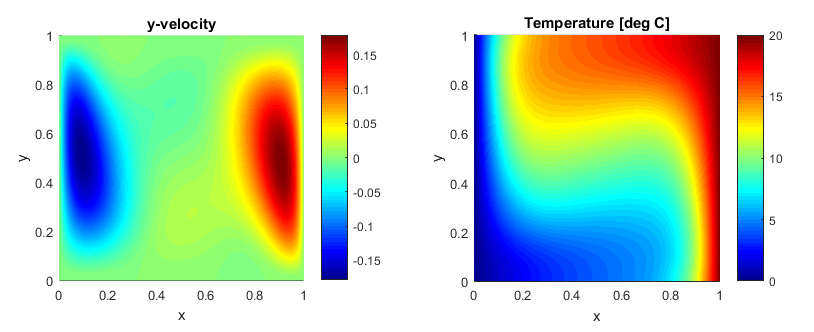
\includegraphics[trim = {1.7cm 2cm 0 1cm}, clip , angle=0, scale=0.50]{NaturalConvectionFromNet}
				\caption{Convecção natural.}
				\end{figure}

		\end{frame}





	\section{Parte 1 : Modelo 2D representativo}
	
	
	\begin{frame} 
	\frametitle{Domínio bidimensional com advecção imposta}
	\begin{minipage}[h!]{0.49\textwidth}
	$\bullet$ Converter código bidimensional antigo em MatLab para c++.\\
	$\bullet$ Desenvolver advecção, com velocidades em $x$ e $y$ impostas para todo o domínio.\\
	$\bullet$ Desenvolver biblioteca visual para este estudo com openGL.\\
	$\bullet$ Converter para o fortran os códigos.\\
	$\bullet$ Experimentar plataforma openGL com fortran.\\
	$\bullet$ Estudar acoplamento velocidade pressão.\\
	\end{minipage}
	\begin{minipage}[h!]{0.49\textwidth}
	\begin{figure}[h!]
		\centering
		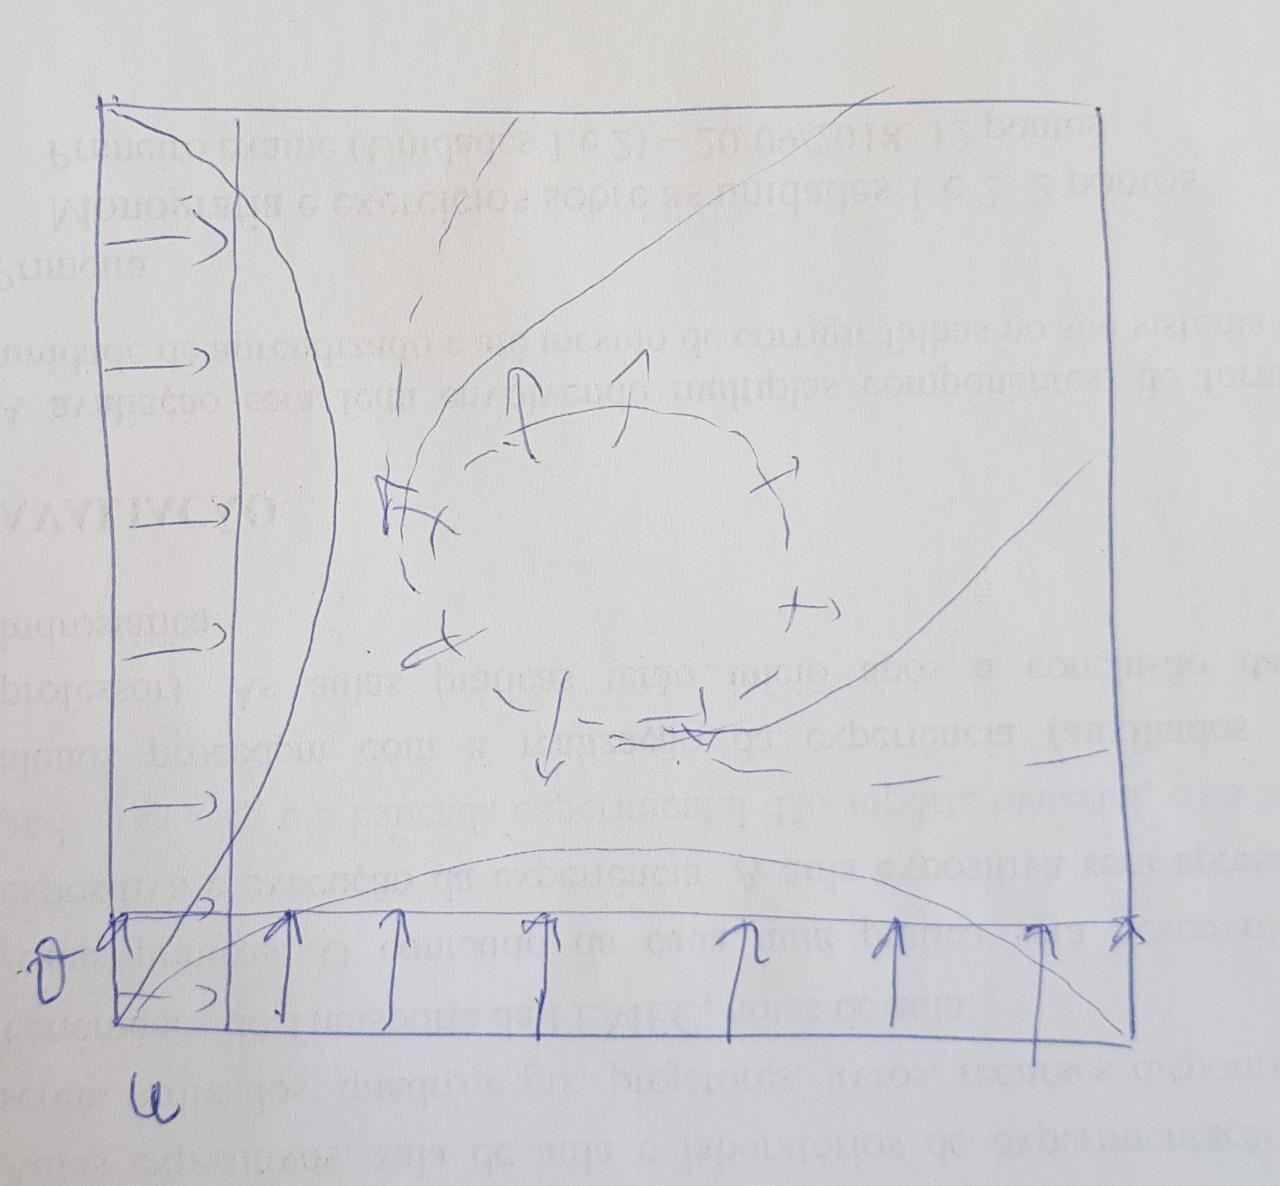
\includegraphics[trim = {0cm 1cm 0 1cm}, clip , angle=0, scale=0.15]{ImagemProfessor1}
		\caption{Esquema do professor.}
	\end{figure}
	\end{minipage}
	\end{frame}
	
	
	
	
	
	
	\begin{frame} 
	\frametitle{Modelo matemático diferencial}
%	\begin{minipage}[h!]{0.49\textwidth}
		$\bullet$ A equação da energia térmica foi desenvolvida como base, com termos advectivos.\\
		$\bullet$ A dimensão $z$ foi ignorada, considerando-se auto similaridade neste eixo.\\
		
%	\end{minipage}
%	\begin{minipage}[h!]{0.49\textwidth}
	
	\begin{equation}
	\frac{\partial T}{\partial t} + u \frac{\partial T}{\partial x} + v \frac{\partial T}{\partial y} = \alpha \left[  \frac{\partial^2 T}{\partial x^2} + \frac{\partial^2 T}{\partial y^2}   \right] 
	\end{equation}
	
%	\end{minipage}
	\end{frame}





	\begin{frame} 
	\frametitle{Modelo numérico explícito}
	%	\begin{minipage}[h!]{0.49\textwidth}
	$\bullet$ Todas as derivadas parciais espaciais de primeira ordem foram discretizadas pelo método de Newton de primeira ordem em diferenças centradas.\\
	$\bullet$ Todas as derivadas parciais de segunda ordem foram discretizadas utilizando-se o método Newton de segunda ordem em diferenças centradas.\\
	$\bullet$ No tempo foi utilizado o método de Euler de primeira ordem.\\
	
	%	\end{minipage}
	%	\begin{minipage}[h!]{0.49\textwidth}
	
	\begin{equation}
	\begin{split}
	\frac{T_{i,j}^{k} - T_{i , j}^{k-1} }{\Delta t}
	= \alpha \left[  \frac{T_{i+1,j}^{k-1} - 2 T_{i,j}^{k-1} + T_{i-1,j}^{k-1} }{\Delta x^2} \right]\\
	+\alpha \left[\frac{T_{i,j+1}^{k-1} - 2 T_{i,j}^{k-1} + T_{i,j-1}^{k-1}}{\Delta y^2}\right] - u \frac{T_{i+1,j}^{k-1} - T_{i-1,j}^{k-1}}{2 \Delta x} - v \frac{T_{i,j+1}^{k-1} - T_{i , j-1}^{k-1}}{2 \Delta y}  
	\end{split}
	\end{equation}
	
	%	\end{minipage}
	\end{frame}

	\begin{frame} 
	\frametitle{Modelo numérico explícito}
	$\bullet$ Com algumas simplificações chega-se na expressão utilizada no código:
	\begin{equation}
	\begin{split}
	T_{i,j}^{k} = T_{i,j}^{k-1} \left( 1 - 4 \frac{\alpha \Delta t}{\Delta s ^2}\right) + T_{i -1, j}^{k-1} \left( \alpha \frac{\Delta t}{\Delta s^2} + u \frac{\Delta t}{2 \Delta s} \right)\\
	+ T_{i,j-1}^{k-1} \left( \alpha \frac{\Delta t}{\Delta s^2} + v \frac{\Delta t}{2 \Delta s} \right) +  T_{i+1,j}^{k-1} \left( \alpha \frac{\Delta t}{ \Delta s^2} - u \frac{\Delta t}{2 \Delta s}\right) \\
	+  T_{i,j+1}^{k-1} \left( \alpha \frac{\Delta t}{\Delta s^2} - v \frac{\Delta t}{2 \Delta s}\right)
	\end{split}
	\end{equation}

	\end{frame}





	\begin{frame} 
	\frametitle{Modelo numérico implícito}
	%	\begin{minipage}[h!]{0.49\textwidth}
	$\bullet$ Todas as derivadas parciais espaciais de primeira ordem foram discretizadas pelo método de Newton de primeira ordem em diferenças centradas.\\
	$\bullet$ Todas as derivadas parciais de segunda ordem foram discretizadas utilizando-se o método Newton de segunda ordem em diferenças centradas.\\
	$\bullet$ No tempo foi utilizado o método de Euler recuado de primeira ordem.\\
	
	%	\end{minipage}
	%	\begin{minipage}[h!]{0.49\textwidth}
	
	\begin{equation}
	\begin{split}
	\frac{T_{i,j}^{k} - T_{i , j}^{k-1} }{\Delta t}
	= \alpha \left[  \frac{T_{i+1,j}^{k} - 2 T_{i,j}^{k} + T_{i-1,j}^{k} }{\Delta x^2} \right]\\
	 +\alpha \left[\frac{T_{i,j+1}^{k} - 2 T_{i,j}^{k} + T_{i,j-1}^{k}}{\Delta y^2}\right] - u \frac{T_{i+1,j}^{k} - T_{i-1,j}^{k}}{2 \Delta x} - v \frac{T_{i,j+1}^{k} - T_{i , j-1}^{k}}{2 \Delta y}  
	\end{split}
	\end{equation}
	
	%	\end{minipage}
	\end{frame}

	\begin{frame} 
	\frametitle{Modelo numérico implícito}
	$\bullet$ Com algumas simplificações chega-se na expressão utilizada no código:
	\begin{equation}
	\begin{split}
	T_{i,j}^{k} = \frac{T_{i,j}^{k-1} + T_{i -1, j}^{k} \left( \alpha \frac{\Delta t}{\Delta s^2} + u \frac{\Delta t}{2 \Delta s} \right) 	+ T_{i,j-1}^{k} \left( \alpha \frac{\Delta t}{\Delta s^2} + v \frac{\Delta t}{2 \Delta s} \right)}{ 1 - 4 \frac{\alpha \Delta t}{\Delta s ^2}} \\
    + \frac{  T_{i+1,j}^{k} \left( \alpha \frac{\Delta t}{ \Delta s^2} - u \frac{\Delta t}{2 \Delta s}\right) 
	+  T_{i,j+1}^{k} \left( \alpha \frac{\Delta t}{\Delta s^2} - v \frac{\Delta t}{2 \Delta s}\right)}{ 1 - 4 \frac{\alpha \Delta t}{\Delta s ^2}}
	\end{split}
	\end{equation}
	
	\end{frame}
	
	
	
	
	
	
	\begin{frame} 
	\frametitle{Código em c++}
	\begin{minipage}[h!]{0.49\textwidth}
	$\bullet$ Foi traduzido do MatLab para c++ o código clássico e implementada as mudanças matemáticas deste novo caso.\\
	$\bullet$ Casos teste foram utilizados para validação qualitativa.\\
	$\bullet$ Alguns parâmetros de teste notáveis foram: \\
	
	- Alpha = 97 (Alumínio) \\
	- u = 5 m/s \\
	- v = 5 m/s \\
	
	$\bullet$ Para o explícito foi obedecida a condição de convergência:
	
	\begin{equation}
	\Delta t \leq \frac{\Delta s ^2}{4 \alpha} 
	\end{equation}
		
	\end{minipage}
	\begin{minipage}[h!]{0.49\textwidth}
		\begin{figure}[h!]
		\centering
		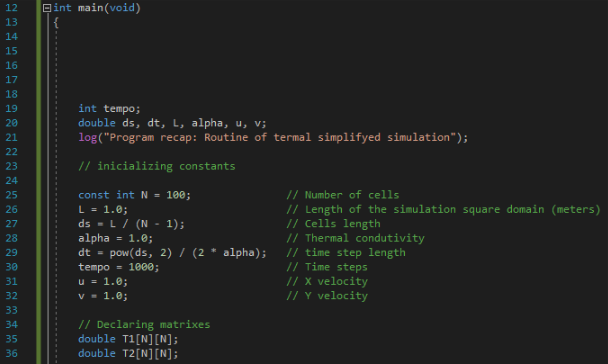
\includegraphics[trim = {0cm 1cm 5cm 1cm}, clip , angle=0, scale=0.65]{printCodigo1}
		\caption{código no editor. Declaração de funções}
	\end{figure}
	\end{minipage}
	\end{frame}
	
	
	
	
	
	
	\begin{frame}
	\frametitle{Resultados iniciais}
	\begin{minipage}[h!]{0.49\textwidth}
	$\bullet$  Inicialmente, foi tratado somente condução térmica, as velocidades foram setadas em zero, resultando na solução da energia térmica clássica. Com a simulação de alguns casos, obteve-se os resultados ao lado.Apesar de se obedecer aos quesitos de convergência, não se consegue desenvolver uma simulação muito grande. E o resultado parece ser dependente da malha.
	\end{minipage}
	\begin{minipage}[h!]{0.49\textwidth}
		\begin{figure}[h!]
			\centering
			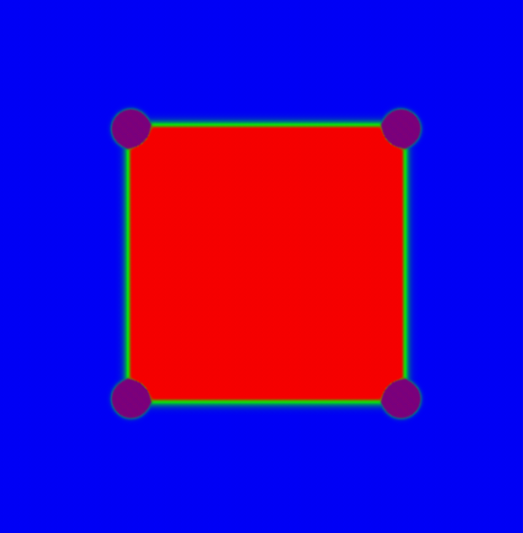
\includegraphics[trim = {1cm 1cm 1cm 1cm}, clip , angle=0, scale=0.45]{preliminar_results_1}
			\caption{Divergência da solução.}
		\end{figure}
	\end{minipage}
	\end{frame}





	\begin{frame}
	\frametitle{Resultados iniciais}
	\begin{minipage}[h!]{0.49\textwidth}
		\begin{figure}[h!]
			\centering
			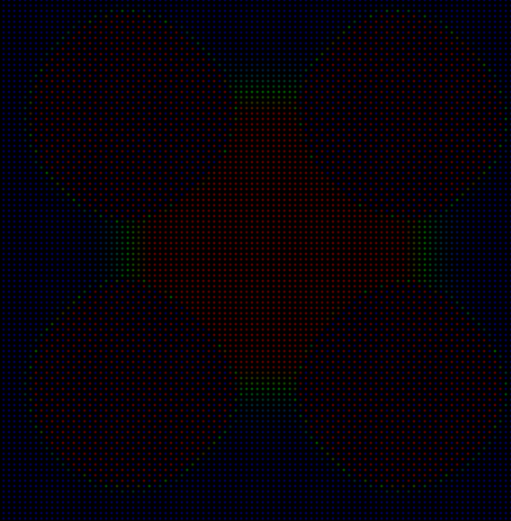
\includegraphics[trim = {1cm 1cm 1cm 1cm}, clip , angle=0, scale=0.38]{preliminar_results_2}
			\caption{Simulação com poucos pontos.}
		\end{figure}
	\end{minipage}
	\begin{minipage}[h!]{0.49\textwidth}
		\begin{figure}[h!]
			\centering
			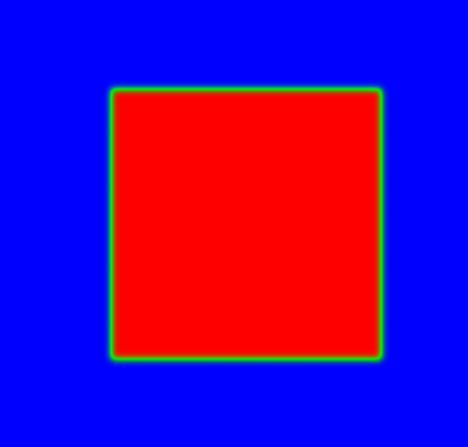
\includegraphics[trim = {1cm 1cm 1cm 1cm}, clip , angle=0, scale=0.45]{preliminar_results_3}
			\caption{Simulação com muitos pontos antes da divergência.}
		\end{figure}
	\end{minipage}
	\end{frame}


	\begin{frame}
	\frametitle{Resultados iniciais}
	
	$\bullet$ Mas, diminuindo-se o passo de tempo a valores muito pequenos, foi possível se alcançar a convergência para longos tempos de simulação, foi então que se observou um erro numérico na determinação do passo de tempo, corrigindo ele, obteve-se:
	
	
	\begin{minipage}[h!]{0.30\textwidth}
		\begin{figure}[h!]
			\centering
			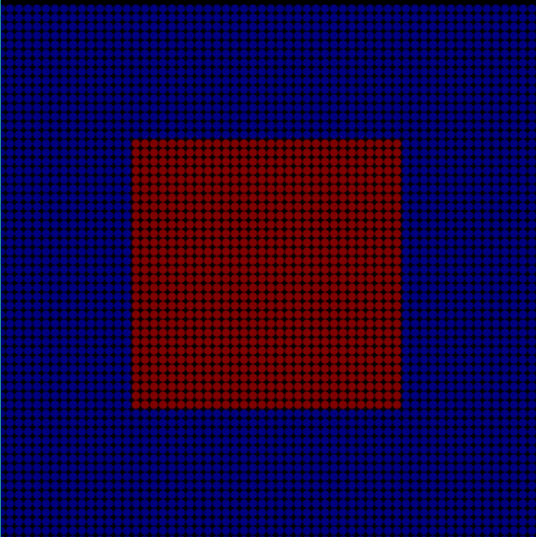
\includegraphics[trim = {1cm 1cm 1cm 1cm}, clip , angle=0, scale=0.3]{sucesso_!}
			\caption{Condição inicial.}
		\end{figure}
	\end{minipage}
	\begin{minipage}[h!]{0.30\textwidth}
		\begin{figure}[h!]
			\centering
			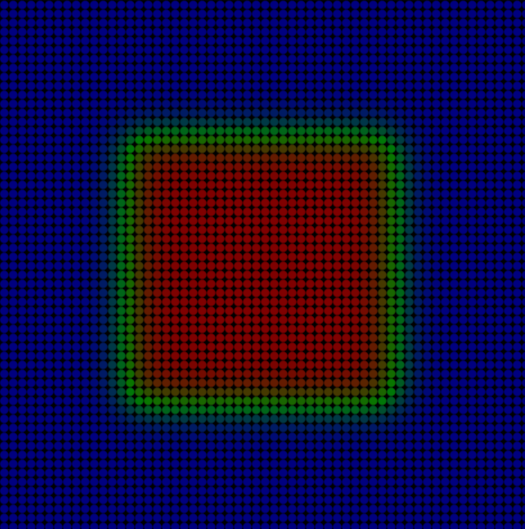
\includegraphics[trim = {1cm 1cm 1cm 1cm}, clip , angle=0, scale=0.3]{sucesso_2}
			\caption{Situação intermediária.}
		\end{figure}
	\end{minipage}
\begin{minipage}[h!]{0.30\textwidth}
	\begin{figure}[h!]
		\centering
		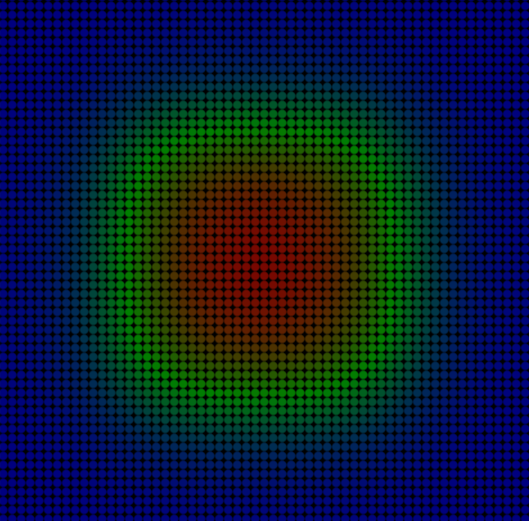
\includegraphics[trim = {1cm 1cm 1cm 1cm}, clip , angle=0, scale=0.3]{sucesso_3}
		\caption{Simulação bem sucedida.}
	\end{figure}
\end{minipage}
	\end{frame}




	\begin{frame}
	\frametitle{Resultados iniciais}
	
	$\bullet$ Tendo-se sucesso no método clássico, acionou-se a velocidade a 5 m/s obtendo-se o seguinte resultado:
	
	
	\begin{minipage}[h!]{0.30\textwidth}
		\begin{figure}[h!]
			\centering
			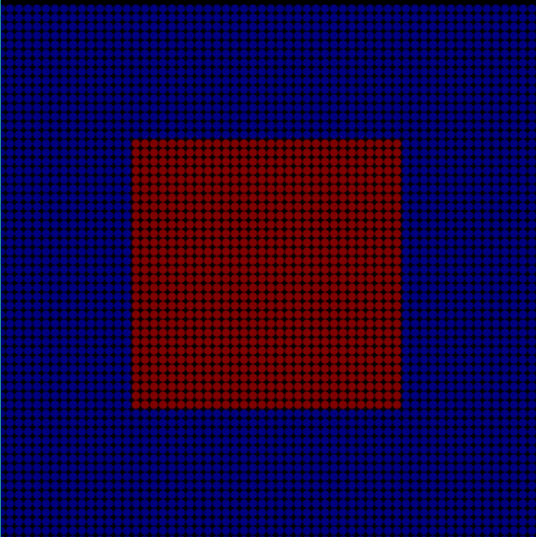
\includegraphics[trim = {1cm 1cm 1cm 1cm}, clip , angle=0, scale=0.3]{sucesso_!}
			\caption{Condição inicial.}
		\end{figure}
	\end{minipage}
	\begin{minipage}[h!]{0.30\textwidth}
		\begin{figure}[h!]
			\centering
			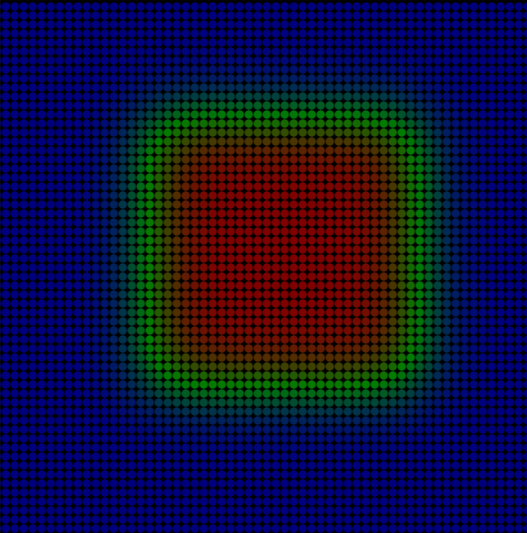
\includegraphics[trim = {1cm 1cm 1cm 1cm}, clip , angle=0, scale=0.3]{sucesso_velocidade_2}
			\caption{Situação intermediária.}
		\end{figure}
	\end{minipage}
	\begin{minipage}[h!]{0.30\textwidth}
		\begin{figure}[h!]
			\centering
			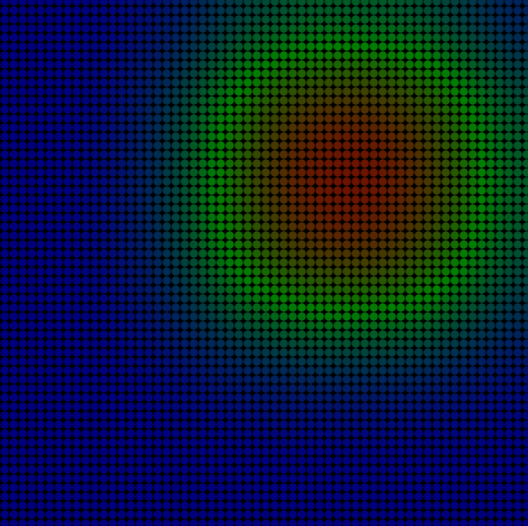
\includegraphics[trim = {1cm 1cm 1cm 1cm}, clip , angle=0, scale=0.3]{sucesso_velocidade_3}
			\caption{Simulação bem sucedida.}
		\end{figure}
	\end{minipage}
\end{frame}	



	\begin{frame}
\frametitle{Validação e análise de erros e convergência}
\begin{minipage}[h!]{0.77\textwidth}
$\bullet$ Com um programa funcional, chegou então a hora de se fazer uma análise de erros a fim de se validar quantitativamente o método. até mesmo com uma análise na ordem de convergência.  \\
$\bullet$ Para isso, utilizou-se do artifício da solução manufaturada, que consiste em se criar um termo fonte e propor uma solução para T, de forma a se desenvolver uma solução exata para a equação quando acrescida deste termo fonte. Seguem a solução proposta e o termo fonte:

\begin{equation}
T = e ^{1 - (x^2 + y^2 + t)}
\end{equation}

\begin{equation}
G = e^{1 - (x^2 + y^2 + t)} \left( 4 \alpha - 2 u x - 2 v y - 4 \alpha (x^2 + y^2) - 1 \right)
\end{equation}

$\bullet$ Assim temos a função analítica a ser analisada pelo método numérico como segue:


	\begin{equation}
\frac{\partial T}{\partial t} + u \frac{\partial T}{\partial x} + v \frac{\partial T}{\partial y} = \alpha \left[  \frac{\partial^2 T}{\partial x^2} + \frac{\partial^2 T}{\partial y^2}   \right] + G 
\end{equation}
\end{minipage}
\begin{minipage}[h!]{0.17\textwidth}
\begin{figure}[h!]
	\centering
	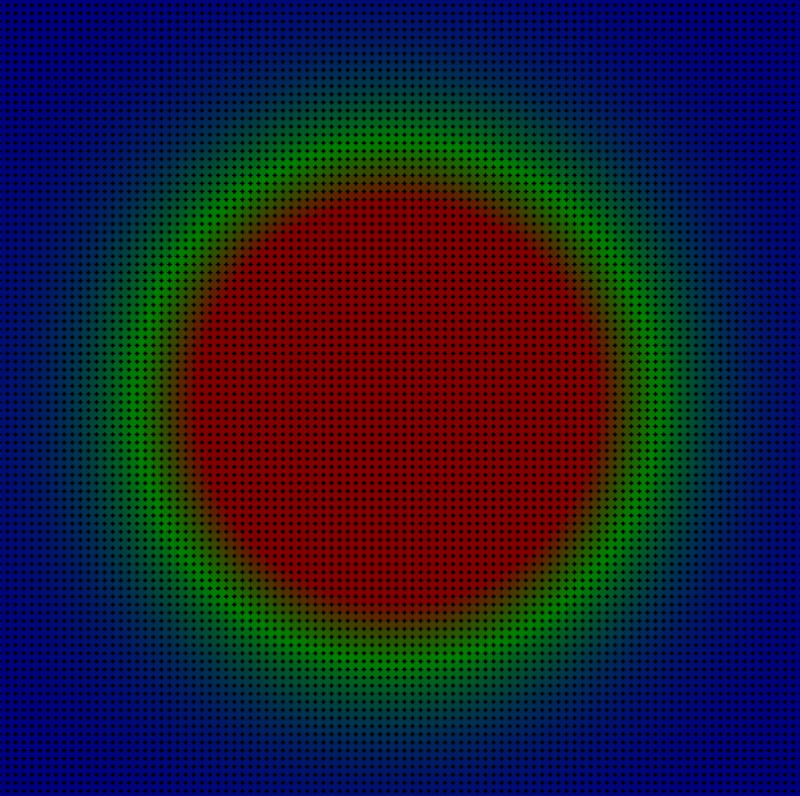
\includegraphics[trim = {0cm 0cm 0cm 0cm}, clip , angle=0, scale=0.1]{Analise_manufaturada}
	\caption{Resultado simulado.}
\end{figure}
\begin{figure}[h!]
	\centering
	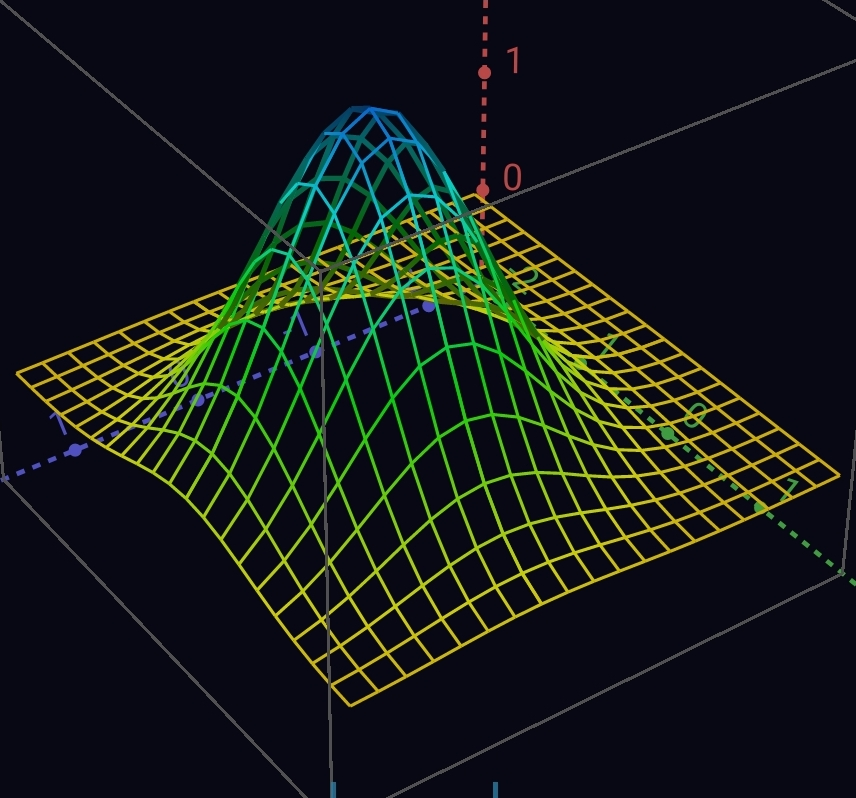
\includegraphics[trim = {0cm 0cm 0cm 0cm}, clip , angle=0, scale=0.07]{resultado_analitico}
	\caption{ Resultado exato.}
\end{figure}
\end{minipage}
\end{frame}	





\begin{frame} 
\frametitle{Modelo numérico explícito}
$\bullet$ Com algumas simplificações chega-se na expressão utilizada no código:
\begin{equation}
\begin{split}
T_{i,j}^{k} = T_{i,j}^{k-1} \left( 1 - 4 \frac{\alpha \Delta t}{\Delta s ^2}\right) + T_{i -1, j}^{k-1} \left( \alpha \frac{\Delta t}{\Delta s^2} + u \frac{\Delta t}{2 \Delta s} \right)\\
+ T_{i,j-1}^{k-1} \left( \alpha \frac{\Delta t}{\Delta s^2} + v \frac{\Delta t}{2 \Delta s} \right) +  T_{i+1,j}^{k-1} \left( \alpha \frac{\Delta t}{ \Delta s^2} - u \frac{\Delta t}{2 \Delta s}\right) \\
+  T_{i,j+1}^{k-1} \left( \alpha \frac{\Delta t}{\Delta s^2} - v \frac{\Delta t}{2 \Delta s}\right) + G
\end{split}
\end{equation}

\end{frame}




\begin{frame} 
\frametitle{Modelo numérico implícito}
$\bullet$ Com algumas simplificações chega-se na expressão utilizada no código:
\begin{equation}
\begin{split}
T_{i,j}^{k} = \frac{T_{i,j}^{k-1} + T_{i -1, j}^{k} \left( \alpha \frac{\Delta t}{\Delta s^2} + u \frac{\Delta t}{2 \Delta s} \right) 	+ T_{i,j-1}^{k} \left( \alpha \frac{\Delta t}{\Delta s^2} + v \frac{\Delta t}{2 \Delta s} \right)}{ 1 - 4 \frac{\alpha \Delta t}{\Delta s ^2}} \\
+ \frac{  T_{i+1,j}^{k} \left( \alpha \frac{\Delta t}{ \Delta s^2} - u \frac{\Delta t}{2 \Delta s}\right) 
	+  T_{i,j+1}^{k} \left( \alpha \frac{\Delta t}{\Delta s^2} - v \frac{\Delta t}{2 \Delta s}\right) + G}{ 1 - 4 \frac{\alpha \Delta t}{\Delta s ^2}}
\end{split}
\end{equation}

\end{frame}



\begin{frame} 
\frametitle{Resultados das simulações}
$\bullet$ Dessa forma, foram conduzidas várias simulações em diferentes CFL`s, de forma a se observar o comportamento do erro a partir destes desenvolvimentos, seguem os resultados: \\

\begin{minipage}[h!]{0.49\textwidth}
\begin{figure}[h!]
	\centering
	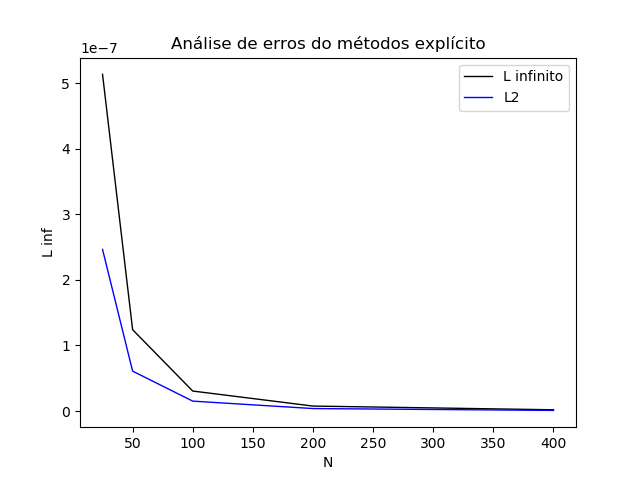
\includegraphics[trim = {0cm 0cm 0cm 0cm}, clip , angle=0, scale=0.4]{analise_de_erros_explicito}
	\caption{ Análise de convergência para o método explicito. Uma análise das normas revelou uma convergência de 2 ordem. Quando se dobrava o numero de células, se dividia por aproximadamente 4 o erro.}
\end{figure}
\end{minipage}
\begin{minipage}[h!]{0.49\textwidth}
\begin{figure}[h!]
	\centering
	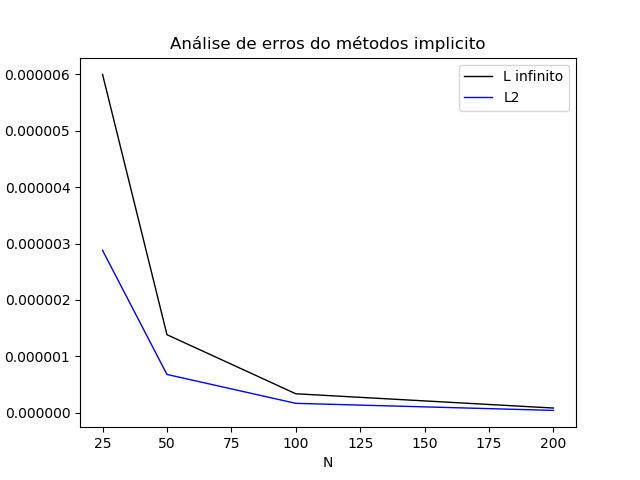
\includegraphics[trim = {0cm 0cm 0cm 0cm}, clip , angle=0, scale=0.4]{analise_de_erros_implicito}
	\caption{ Análise de convergência para o método implícito. Uma análise das normas revelou uma convergência de 2 ordem. Quando se dobrava o numero de células, se dividia por aproximadamente 4 o erro.}
\end{figure}
\end{minipage}
\end{frame}






\begin{frame} 
\frametitle{Acoplamento velocidade pressão }
$\bullet$ Dessa forma, foram conduzidas várias simulações em diferentes CFL`s, de forma a se observar o comportamento do erro a partir destes desenvolvimentos, seguem os resultados: \\


\end{frame}


	
	

	
	\section{Parte 2 : Modelo 3D representativo}
	
	

	
	
	\section{Agradecimentos}
		
		
		
		
		
			\begin{frame}
				\placelogomflab 
				\frametitle{Agradecimentos}
				\begin{figure}
					\begin{center}
						\begin{tabular}{c c}
							{
\includegraphics[trim=0.0cm 0.0cm 0.0cm 0.0cm,clip=true,height=0.2\textheight]{figuras/petrobras.png}}&{
\includegraphics[trim=0.0cm 0.0cm 0.0cm 0.0cm,clip=true,height=0.2\textheight]{figuras/logo_mflab.png}}\\
							{
\includegraphics[trim=0.0cm 0.0cm 0.0cm 0.0cm,clip=true,height=0.2\textheight]{figuras/cnpq.png}}&{
\includegraphics[trim=0.0cm 0.0cm 0.0cm 0.0cm,clip=true,height=0.2\textheight]{figuras/CAPES.png}}\\
							{
\includegraphics[trim=0.0cm 0.0cm 0.0cm 0.0cm,clip=true,height=0.2\textheight]{figuras/FAPEMIG.jpg}}&{
\includegraphics[trim=0.0cm 0.0cm 0.0cm 0.0cm,clip=true,height=0.2\textheight]{figuras/UFU_black.jpg}}\\
						\end{tabular}
					\end{center}
				\end{figure}
			\end{frame}
			
			
			
			
			
			\begin{frame}
				\placelogomflab 
				\frametitle{Agradecimentos}
				\fontsize{44pt}{7.2}\selectfont
				\begin{center}
					Obrigado.
				\end{center}
			\end{frame}
		
		
		
		
\end{document}




		



%%%%%%%%%%%%%%%%%%%%%%%%%%%%%%%%%%%%%%% Exemplo de formatação de imagens		
%		\begin{frame}
%			\frametitle{Adição de fronteiras extras}
%			\begin{tabular}{c c}
%				
%				{\includegraphics[trim=0.0cm 0.0cm 0.0cm 0.0cm,clip=true,loop,height=0.5\textheight]{figuras/filtration_depois.png}}&{\includegraphics[trim=0.0cm 0.0cm 0.0cm 0.0cm,clip=true,loop,height=0.4\textheight]{figuras/filtration_depois_zoom.png}}\\
%				
%			\end{tabular}
%			
%		\end{frame}




%%%%%%%%%%%%%%%%%%%%%%%%%%%%%%%%%%%%%% Exemplo de formatação de imagens		
%		\begin{frame}
%			\frametitle{Agora}
%			\centering
%			\begin{tabular}{c}
%				
%				{\includegraphics[trim=0.00cm 2.0cm 0.0cm 2.0cm,clip=true,loop,width=0.9\textwidth]{figuras/t_x_51f.png}}\\{\includegraphics[trim=0.01cm 0.0cm 0.01cm 0.0cm,clip=true,loop,width=0.9\textwidth]{figuras/t_x_51999.png}}\\{\includegraphics[trim=0.01cm 0.0cm 0.01cm 0.0cm,clip=true,loop,width=0.9\textwidth]{figuras/t_x_51999g.png}}\\{\includegraphics[trim=0.01cm 0.0cm 0.01cm 0.0cm,clip=true,loop,width=0.9\textwidth]{figuras/t_x_51999y.png}}\\{\includegraphics[trim=0.01cm 0.0cm 0.01cm 0.0cm,clip=true,loop,width=0.9\textwidth]{figuras/t_x_51999b.png}}
%				
%			\end{tabular}
%			
%		\end{frame}





%%%%%%%%%%%%%%%%%%%%%%%%%%%%%%%%%%%%%  Formatação de equações:		
%		\begin{frame}
%			\frametitle{Newton-Raphson}
%			
%			\flushleft
%			Método de interface com jacobiano composto:
%			
%			\centering
%			\begin{equation}\label{forte_eqNewton}
%			K(D+\Delta D) \approx K(D)+\Delta D \, J(D)
%			\end{equation}
%			\begin{equation}\label{forte_eqNewton2}
%			K(D) =  Estrutura(Fluido(D))-D =  0
%			\end{equation}
%			\begin{equation}\label{forte_eqNewton3}
%			J(D) =  Estrutura'(Fluido(D)) \, Fluido'(D)-I
%			\end{equation}
%			\begin{equation}\label{forte_eqNewton4}
%			Fluido(D): \mathbb{R}^{n} \to \mathbb{R}^{m}
%			\end{equation}
%			
%			\flushleft
%			$Fluido'(D)$ é de tamanho $m x n$
%			
%			\centering
%			
%			\begin{equation}\label{forte_eqNewton5}
%			Estrutura(F): \mathbb{R}^{m} \to \mathbb{R}^{n}
%			\end{equation}
%			
%			\flushleft
%			$Estrutura'(F)$ é de tamanho $n x m$\\
%			$Estrutura'(Fluido(D)) \, Fluido'(D)$ e $I$ é de tamanho $n x n$
%		\end{frame}




%%%%%%%%%%%%%%%%%%%%%%%%%%%%%%%%%%%%%%%%%%% Vários exemplos de formatação textual:		


%		\begin{frame}
%			\frametitle{Conveniência do método de Multi Direct Forcing}
%			
%			\flushleft
%			\textbf{Fraco:}\\
%			$\bullet$ Predição da velocidade.\\
%			$\bullet$ MDF. (Imposição da condição de dirichlet na interface e cálculo da força)\\
%			$\bullet$ Estrutura.\\
%			$\bullet$ Poisson.\\
%			$\bullet$ Correção de velocidade e pressão.\\ \\
%
%			\textbf{Forte:}\\
%			$\bullet$ Predição da velocidade.\\
%			while \\
%			\quad	$\longrightarrow$ MDF.\\
%			\quad	$\longrightarrow$ Estrutura.\\
%			end\\
%			$\bullet$ Poisson.\\
%			$\bullet$ Correção de velocidade e pressão.\\
%
%		\end{frame}

		

%		
%%%%%%%%%%%%%%%%%%%%%%%%%%%%%%%%%  Modelo duas fotos lado a lado:


%		\begin{frame}
%		\frametitle{Limite do fraco}
%			ct=121
%			mi=200
%			\begin{tabular}{c c}
%			{\includegraphics[width=0.45\linewidth]{../../simulacoes_Estudo_dirigido2/fraco_mi_200_0_15_ct141/figuras/estrutura/vel_151}}&
%		   {\includegraphics[width=0.45\linewidth]{../../simulacoes_Estudo_dirigido2/fraco_mi_200_0_15_ct141/figuras/estrutura/vel_251}}\\
%		   {(a) Velocidade em linha centro da estrutura} & {(b) Velocidade transversal centro da estrutura}
%		\end{tabular}
%		\end{frame}



%%%%%%%%%%%%%%%%%%%%%%%%%%%%%%%%%%  Modelo tabela :

%		\begin{frame}
%			\frametitle{Comparação número de iterações}
%			\begin{tabular}{c c c c}
%				\hline
%				Método & Mínimo     &    Máximo &  Média\\ \hline
%				FPI MDF variável & 8     &    101 &  8.9764764764764760\\
%				FPI MDF fixo & 8     &     11 &  8.9099099099099099\\
%				QN Primeiro método de Broyden MDF variável & 18    &     101 &  18.281281281281281 \\ \hline
%			\end{tabular}
%		\end{frame}	




